\documentclass[10pt]{article}
\usepackage[a4paper,margin=2.0cm]{geometry}
\usepackage[T1]{fontenc}
\usepackage{lmodern}
\usepackage{microtype}
\usepackage{amsmath}
\usepackage{booktabs}
\usepackage{graphicx}
\usepackage{caption}
\usepackage{float}
\usepackage[hidelinks]{hyperref}
\graphicspath{{figures/}}
\setlength{\parskip}{0.45em}
\setlength{\parindent}{0pt}
\captionsetup{font=small,labelfont=bf}

\title{\vspace{-1.6em}Multi-codec: CodecLeafAlias with VP9, HEVC and AV1 partitions\\ under standard encoder configurations}
\author{}
\date{\vspace{-2.4em}}

\begin{document}
\maketitle
\vspace{-1.0em}

\textbf{Summary.} CodecLeafAlias needs only two things from a codec: a block partition whose blocks follow image content, and the mean of each block. Every block-based codec provides both, so the method is not tied to VP9 or to its variance partitioning mode. With VP9-, HEVC- and AV1-style partitions, under the rate-distortion (RD) search of a standard configuration, the rendered error stays within 3--4\% of the paper's partition at usual quantizers and within about 7\% at the coarsest, provided the tree of each predicted frame is taken from the last keyframe and carried along the motion vectors. With weights from real VP9, HEVC and AV1 encodes, the error stays within 3\% across bitrates.

\section*{1\quad What the method takes from a codec}

The paper forces VP9's variance partitioning, so that block sizes follow the variance of the image. A standard configuration instead chooses blocks by RD search, and every codec family does this with its own block sizes: VP9 from 64 to 8 pixels with rectangular splits, HEVC from 64 to 8 pixels with a pure quadtree, AV1 from 128 to 4 pixels with rectangular splits. In an intra-coded frame (a keyframe), the RD search splits where the image is detailed and keeps large blocks where it is smooth, which is what the light sampler needs. In a predicted frame, the RD search runs on the residual left after motion compensation, so its blocks follow \emph{prediction error} rather than image content. Where motion is predicted well, a detailed region can be coded as one large block.

\textbf{Keyframe tree carried along the motion vectors.} The paper's workaround for standard configurations is to use, for every predicted frame, the partition of the last keyframe, moved along the block motion vectors of the stream. The keyframe tree follows content; the motion vectors keep it aligned with the content as it moves. We evaluate this against the two simpler alternatives: using the predicted frame's own RD tree directly, and reusing the keyframe tree without moving it. Figure~\ref{fig:trees} shows the partitions on one frame.

\begin{figure}[H]
\centering
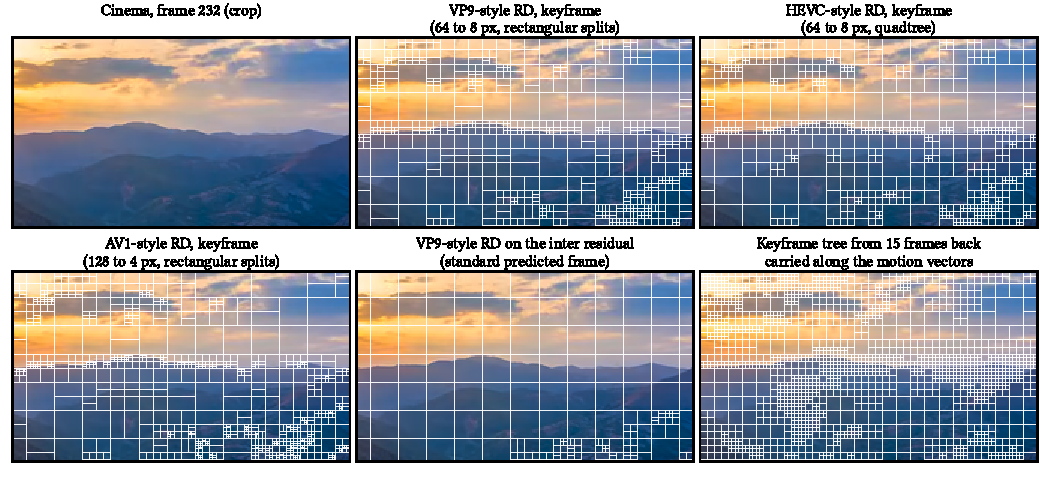
\includegraphics[width=\linewidth]{codec_trees_cinema.pdf}
\caption{Partitions of a Cinema frame at quantizer 64 of 1023. Keyframe RD trees of the three codec families follow content: small blocks along the ridges and in the textured hills, large blocks in the smooth sky. The RD tree of a predicted frame (bottom middle) follows prediction error instead and leaves most of the hills in large blocks. The keyframe tree carried along the motion vectors (bottom right) follows content again.}
\label{fig:trees}
\end{figure}

\section*{2\quad Setup}

Five scenes of the paper (Rover, Cinema, Fireplace, Phone, Convergence), two frames each, in 10-bit PQ (BT.2100). For each codec family we reproduce its partition search on the frames, with its block sizes and split modes, at three quantizers: 16, 64 and 256 of 1023 code values (fine, usual, very coarse). Partition sources: the VP9 variance mode of the paper; the RD tree of a predicted frame, on its motion-compensated residual; the last keyframe's tree reused as is (keyframe interval 15 frames); and the last keyframe's tree carried along the motion vectors. To isolate the partition, every leaf gets its exact mean radiance. Each configuration is rendered in our GPU path tracer at equal samples (4 spp, 8 captures) and compared with a converged reference. We report RMSE relative to the paper's CodecLeafAlias partition on the same frames.

\section*{3\quad Results}

\begin{table}[H]
\centering\small
\begin{tabular}{lccccccccc}
\toprule
& \multicolumn{3}{c}{Quantizer 16} & \multicolumn{3}{c}{Quantizer 64} & \multicolumn{3}{c}{Quantizer 256} \\
\cmidrule(lr){2-4}\cmidrule(lr){5-7}\cmidrule(lr){8-10}
Partition source & VP9 & HEVC & AV1 & VP9 & HEVC & AV1 & VP9 & HEVC & AV1 \\
\midrule
RD tree of a predicted frame & 1.032 & 1.034 & 1.073 & 1.118 & 1.120 & 1.219 & 1.135 & 1.136 & 1.243 \\
Keyframe tree, reused & 1.049 & 1.049 & 1.043 & 1.059 & 1.066 & 1.054 & 1.099 & 1.104 & 1.112 \\
\textbf{Keyframe tree + motion vectors} & \textbf{1.025} & \textbf{1.034} & \textbf{1.030} & \textbf{1.028} & \textbf{1.030} & \textbf{1.042} & \textbf{1.054} & \textbf{1.066} & \textbf{1.054} \\
\midrule
VP9 variance mode (paper) & 1.037 & & & 1.047 & & & 1.135 & & \\
\bottomrule
\end{tabular}
\caption{Worst RMSE over the five scenes, relative to the paper's CodecLeafAlias partition. Lower is better; 1 means equal.}
\label{tab:worst}
\end{table}

\begin{table}[H]
\centering\small
\begin{tabular}{llccccc}
\toprule
Quantizer & Codec family & Rover & Cinema & Fireplace & Phone & Convergence \\
\midrule
16 & VP9 & 1.014 & 1.007 & 1.025 & 1.011 & 1.017 \\
& HEVC & 1.034 & 1.011 & 1.031 & 1.027 & 1.020 \\
& AV1 & 1.005 & 1.007 & 1.030 & 1.017 & 1.009 \\
\midrule
64 & VP9 & 1.016 & 1.006 & 1.021 & 1.028 & 1.022 \\
& HEVC & 0.996 & 1.002 & 1.023 & 1.001 & 1.030 \\
& AV1 & 1.042 & 1.017 & 1.026 & 1.030 & 1.015 \\
\midrule
256 & VP9 & 1.022 & 1.011 & 1.025 & 1.021 & 1.054 \\
& HEVC & 1.022 & 1.010 & 1.033 & 1.035 & 1.066 \\
& AV1 & 1.004 & 1.006 & 1.029 & 0.992 & 1.054 \\
\bottomrule
\end{tabular}
\caption{Keyframe tree carried along the motion vectors, per scene. For comparison, BudgetLeafAlias with 4000 leaves gives 1.043, 1.016, 1.035, 1.032 and 1.016 on the same frames.}
\label{tab:kfmv}
\end{table}

\textbf{The three codec families behave alike.} For every partition source, VP9-, HEVC- and AV1-style trees give errors within a few percent of each other (Table~\ref{tab:worst}).

\textbf{Predicted frames need the keyframe tree.} Using a predicted frame's own RD tree costs up to 12\% for VP9 and HEVC and 22\% for AV1 at quantizer 64, and 24\% at 256, because those blocks follow prediction error (Figure~\ref{fig:trees}). Reusing the keyframe tree without moving it is better but drifts as the content moves: up to 6\% at quantizer 64 and 11\% at 256.

\textbf{Carrying the keyframe tree along the motion vectors solves both.} It is the best predicted-frame option, or tied for best, in every column of Table~\ref{tab:worst}: within 2.5--4.2\% of the paper's partition at quantizers 16 and 64 for all three codec families, and within 5.4--6.6\% at quantizer 256. Per scene (Table~\ref{tab:kfmv}), at quantizers 16 and 64 it stays within the range of BudgetLeafAlias, which uses no codec data at all. The motion vectors are part of every coded predicted frame, so this costs no extra analysis.

\textbf{Real encodes.} Weights from real encodes behave the same across codec families. With leaf means from libvpx-vp9, x265 and SVT-AV1 encodes of the same scenes at ten rate points (0.6--74\,Mb/s, decoded PSNR 32--51\,dB), the RMSE stays within 3\% of exact weights, and the worst cases per codec are 1.020 (VP9), 1.015 (HEVC) and 1.029 (AV1) (see the companion note on compression).

\section*{4\quad Conclusion}

CodecLeafAlias does not depend on VP9 or on forcing its variance mode. Partitions in the style of VP9, HEVC and AV1, chosen by the RD search of a standard configuration, work equally well when keyframe trees are used for intra frames and carried along the motion vectors for predicted frames: within 3--4\% of the paper's partition at usual quantizers, and comparable to a partition built without any codec data. Weights from real encodes of all three codecs add at most 3\%.

\end{document}
